\section{Break, Merge and Sort}
\label{sec:g-break-merge}
\source{ICPC 2020--21 Amritapuri Preliminary, problem 3 (PYQ)}{Medium}

\begin{reconbox}
The original statement is no longer online (it was hosted on CodeDrills, which
is offline, and the Notion archive stores only the official \emph{solution
slides}). The statement below is reconstructed from those slides. The cost
model was checked by an exhaustive Dijkstra search over all split/merge
sequences on 300 random arrays: it reproduces the editorial's formula exactly.
Verify against the original if you find it.
\end{reconbox}

\problemstatement{An array $A$ of length $n$. You may \textbf{split} an array
into two contiguous non-empty parts, paying the length of the shorter part,
and \textbf{merge} two sorted arrays into one sorted array, paying the sum of
their lengths. Starting from $A$, obtain a single sorted array with minimum
total cost.}

\begin{patternbox}
Four greedy insights from the editorial: (1) all splits can be done before
all merges; (2) cut exactly at the descents $A_i>A_{i+1}$; (3) peel the
smaller end piece each time; (4) merge the two shortest arrays (Huffman).
\end{patternbox}

\subsection*{Approach and intuition}

Cutting at every descent leaves the maximal sorted runs $r_1,\dots,r_t$;
further cuts only create more merging work.

\textbf{Splitting.} Repeatedly cut off the smaller of the two end runs. Each
cut costs at most that run's length and every run except the largest is cut
off once, so splitting costs $n-\max_i r_i$ --- and this is also a lower
bound.

\textbf{Merging.} Merging behaves like building a Huffman tree: a run merged
$c_i$ times contributes $c_i\cdot r_i$, where $c_i$ is its depth in the merge
tree. As in Huffman coding, there is an optimal tree in which the two
shortest runs are siblings, so ``always merge the two shortest'' is optimal.

\begin{center}
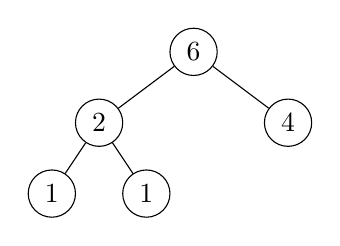
\begin{tikzpicture}[level distance=0.9cm,
  every node/.style={draw,circle,minimum size=0.6cm,inner sep=1pt},
  level 1/.style={sibling distance=2.4cm},
  level 2/.style={sibling distance=1.2cm}]
\node {6}
  child {node {2} child {node {1}} child {node {1}}}
  child {node {4}};
\end{tikzpicture}
\qquad
\begin{minipage}{6.5cm}\small
Runs $1,1,4$: merge $1+1$ (cost $2$), then $2+4$ (cost $6$): merging
cost $8$ = $\sum$ internal nodes.
\end{minipage}
\end{center}

\begin{ideabox}[Total Cost]
\[
  \text{answer}=\bigl(n-\max_i r_i\bigr)+\text{Huffman}(r_1,\dots,r_t).
\]
\end{ideabox}

\subsection*{Algorithm}
\begin{algorithmic}[1]
\State split $A$ into maximal non-decreasing runs $r_1..r_t$
\State $cost\gets n-\max r$; push all $r_i$ into a min-heap
\While{heap size $>1$} \State pop $x,y$; $cost\gets cost+x+y$; push $x+y$ \EndWhile
\State \Return $cost$
\end{algorithmic}

\dryrun{$A=[3,1,4,2]$: runs $[3],[1,4],[2]$, lengths $1,2,1$. Split cost
$4-2=2$. Huffman: $1+1=2$ (cost $2$), $2+2=4$ (cost $4$). Total $8$. A sorted
array has one run and costs $0$. \checkmark}

\subsection*{C++17 implementation}
\cppfile{greedy/27_break_merge_and_sort.cpp}

\begin{complexitybox}
\textbf{Time:} $O(n\log n)$. \textbf{Space:} $O(n)$.
\end{complexitybox}

\begin{pitfallbox}
\begin{itemize}
  \item Equal neighbours are \emph{not} a descent (non-decreasing runs).
  \item Merging runs left-to-right is the classic wrong answer: lengths
        $1,1,1,100$ merged left to right cost $2+3+103=108$; Huffman also
        gives $108$ here, but for $100,1,1,1$ left to right costs
        $101+102+103=306$ vs Huffman $2+3+103=108$.
\end{itemize}
\end{pitfallbox}
